\documentclass{article}
\usepackage{amsmath,amssymb}
\usepackage{hyperref}
\usepackage{graphicx}

\title{\bf{Laboratory Project Two: Calibration of an Oriface Meter}}
\author{Jon Langston \& Nicholas Malaya \& Owen O'Neal \\ Department of Mechanical Engineering \\ University of Texas at Austin} \date{}

\begin{document}
\maketitle
\date{}
\newpage
\section{Presentation of Calibration Data}

\textbf{A calibration of the $C_d$ vs $Re$ and comment on whether your results were as expected.}  

\begin{figure}[!htb]
  \begin{center}
    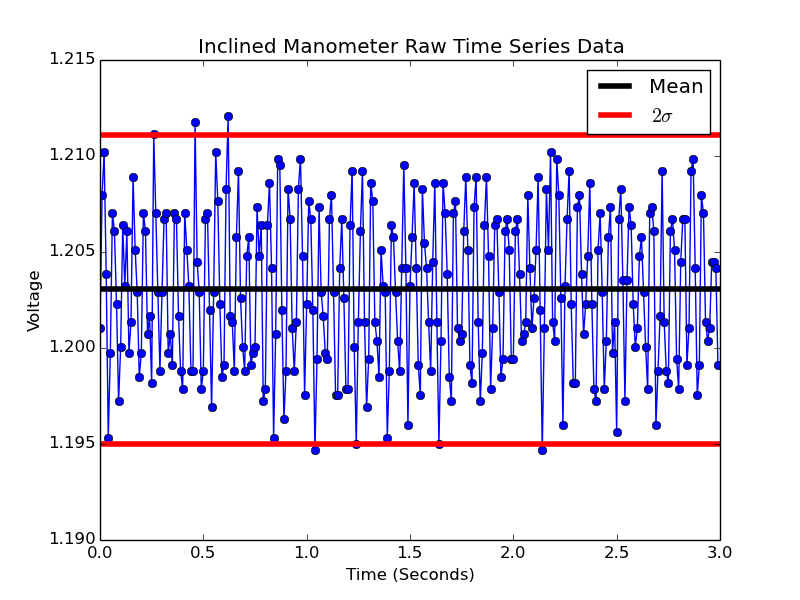
\includegraphics[width = 12 cm]{figs/oriface_time.png}
    \caption{Example raw time series data from a single oriface meter 
      run. The calculated mean of the signal is shown in black, along with
      the two $\sigma$ (standard deviation) confidence interval in
      red.}
    \label{oriface-time}
  \end{center}
\end{figure}

\newpage
\section{Uncertainty Analysis}

\textbf{Uncertainty of flow rate measured using the orifice meter with your calibration.}



\end{document}
